% =====================================================================
\section{Coverage Matrix and Extended Limitations}
\label{app:cov}

\paragraph{Explicit coverage matrix.}
Table~\ref{tab:coverage_full} provides the explicit per-(probe, model)
coverage map; every cell that is not a clean ``run'' is foot-noted with the
reason (API error, unparseable-output, intentional scoping). All quantitative
claims in the main paper are scoped to fully-run (probe, model) cells;
\omini{} appears in main-paper figures and tables only where we have valid
data, and is shown as explicit n/a cells elsewhere.

\begin{table}[t]
  \centering
  \small
  \caption{Explicit per-(probe, model) coverage. All five models are fully
  run on Probe~1 and on GSM/ALGO Probe~2--3 except where footnoted. Strict-PDDL
  BW Probe-2 is n/a for Gemini and \omini{} (protocol aborts at 84--100\% on
  the three models we ran); the NL-tolerant BW Probe-2 rerun covers those
  same three models only (Claude, GPT-4o, Llama).
  $^a$\omini{} GSM Probe~2: 43/44 Phase-1 declarations parse; CCI/TEP computed
  on the parseable subset. $^b$BW interactive PDDL not run on Gemini or
  \omini{} (protocol aborts at $\geq 84\%$ on the three models we did run);
  NL-tolerant BW Probe-2 likewise covers only those three models.
  $^c$GPT-4o/Llama Probe-1 GSM: 20/44 bank-valid (GSM\_001--020 only);
  GSM\_041--064 pending API credit gap fill. $^d$\omini{} ALGO Phase-1
  declaration file absent $\Rightarrow$ ALGO CCI NOT\_COMPUTABLE.}
  \label{tab:coverage_full}
  \begin{tabular}{lccccc}
    \toprule
    & Claude & GPT-4o & Llama & Gemini & \omini \\
    \midrule
    P1 GSM            & 44/44 & 20/44$^c$ & 20/44$^c$ & 44/44 & 44/44 \\
    P1 ALGO           & 110/110 & 110/110 & 110/110 & 110/110 & 110/110 \\
    P1 BW             & 65/65 & 65/65 & 65/65 & 65/65 & 65/65 \\
    P2 GSM (CCI/TEP)  & 44/44 & 44/44 & 44/44 & 44/44 & 43/44$^a$ \\
    P2A ALGO normal   & 110 & 110 & 110 & 110 & 110 \\
    P2A elicited      & 61 & 110 & 61 & 61 & 110 \\
    P2B plausible     & 61 & 61 & 61 & 61 & 61 \\
    P2B implausible   & 61 & 61 & 61 & 61 & 61 \\
    P2 BW (CCI)       & 50 & 50 & 50 & n/a$^b$ & n/a$^b$ \\
    P2 BW NL-tolerant & 50 & 50 & 50 & n/a$^b$ & n/a$^b$ \\
    P3 contam.\ (VRI) & \checkmark & \checkmark & \checkmark & \checkmark & \checkmark \\
    P3 contam.\ (CCI) & \checkmark & \checkmark & \checkmark & \checkmark & n/a$^d$ \\
    \midrule
    P3 mech. & \multicolumn{5}{c}{Qwen/Llama pilots only (Appendix~\ref{app:mech})} \\
    \bottomrule
  \end{tabular}
\end{table}


\paragraph{Extended scoping decisions and future-work pointers.}
\begin{enumerate}
  \item \textbf{Probe-3 as proximity proxy by design.} Training-corpus ground
  truth is unavailable for closed-weight models. We present Infini-gram
  overlap on The Pile/DCLM as an explicitly labelled public-corpus proximity
  proxy and require three-signal convergence before applying a
  retrieval-consistent label.
  \item \textbf{Matched-subset sample sizes are deliberate, not
  under-powered.} We report matched-canonical tests on the subsets where
  matching yields useful $n$ (shortest-path $n{=}34$, coin-change $n{=}10$).
  The full-subtype ALGO CIs are cluster bootstrap over clone families
  (10k, seed 42); GSM/BW use Wilson. The matched tests
  are supporting evidence. The CC inversion ($n{=}10$) is explicitly labelled
  exploratory in the main text.
  \item \textbf{WIS exposure-difficulty co-variance.} WIS is both lower
  exposure and harder---a known property of the algorithm class, not an
  oversight. We treat exposure as a co-occurring signal and flag the confound
  wherever the within-ALGO gradient is cited; a difficulty-matched WIS bank
  is a natural next experiment.
  \item \textbf{CCI is a behavioural metric by construction.} CCI measures
  declared-vs-executed numeric agreement under hard session isolation; it
  deliberately does not probe internal reasoning, which we address separately
  via the Qwen-2.5-7B residual-stream pilot (Appendix~\ref{app:mech}).
  \item \textbf{Cross-tokeniser evidence is built into the design.} Claude
  (BPE-A) and GPT-4o (BPE-B) tokenise the same nonce vocabulary differently
  yet show opposite fragility patterns on the same problem set---this rules
  out tokenisation as the sole driver. A direct tokeniser ablation is a clean
  follow-up.
  \item \textbf{Released artefacts.} The audit bundle ships per-instance
  verifier logs (the single source of truth) plus one legacy derived
  per-problem export, retained only for traceability; no main-paper table or
  figure depends on it.
  \item \textbf{Reasoning-trained breadth.} We chose to run one
  reasoning-trained provider (\omini) at full coverage rather than two at
  partial coverage. Section~\ref{sec:proximity}'s proximity-link observation
  is therefore one-model-strong by design; replicating on
  DeepSeek-R1~\citep{guo2025deepseek} or Qwen3 is the targeted next sweep.
  \item \textbf{Blocksworld protocol evolution.} The strict-PDDL protocol
  revealed a measurement-level finding: interactive PDDL evaluation is brittle
  at the API level. The NL-tolerant rerun canonicalises the BW Probe-2 result;
  the strict-protocol abort taxonomy is reported as a separate methodological
  finding rather than as per-model behavioural CCI.
  \item \textbf{Algorithm-invocation causality.} The five-model elicitation
  experiment establishes an associational null; proving the absence of
  causation requires controlled-prompt RCTs---a clean follow-up.
  \item \textbf{Probe-2 BW coverage decision.} Once the strict-PDDL protocol
  aborted at $\geq 84\%$ on three models, the responsible call was not to
  extend a known-broken measurement to two more. The BW Probe-2 behavioural
  conclusion is driven by the NL-tolerant standard$\to$mystery contrast,
  which covers all five models.
\end{enumerate}

% =====================================================================
\section{Variant Generation Protocol}
\label{app:variants}

\textbf{W1 (paraphrase).} Problem statement rewritten in different words; all
numeric values, entities, and structural relationships preserved exactly.

\textbf{W2 (format change).} Prose converted to structured table, edge list,
interval table, or equation as appropriate to the family (e.g., SP problems
expressed as a weighted adjacency matrix).

\textbf{W3 (entity rename).} All entity identifiers replaced with nonce
tokens drawn from a held-out vocabulary: length-matched,
tokenization-equivalent where feasible (single-token for single-token
originals), and vocabulary-disjoint from the original. Claude (BPE-based) and
GPT-4o (a different BPE variant) show opposite W3 fragility directions on the
same SP and CC subtypes, ruling out a tokenizer-artifact explanation as the
sole driver.

\textbf{W4 (formal notation).} LaTeX equations (GSM); PDDL-like formal
predicates (BW); mathematical edge-list notation (SP/WIS).

\textbf{W5 (direction reversal).} BW: goal and initial states swapped. GSM:
forward problems inverted to backward form (``what was the original amount?''
instead of ``how much remains?''). SP: source and destination nodes swapped,
testing whether the model re-solves from scratch or retrieves a cached
forward solution. W5 is not applied to CC or WIS (no meaningful reversal
exists for those optimization problems).

\textbf{W6 (procedural regeneration).} Same algorithm and parameter ranges;
completely new numeric values.

All variants pass the same domain-specific verifier as the canonical problem
before any model is queried (PDDL simulator for BW; exact-match for GSM;
DP-optimal solver for ALGO).

% =====================================================================
\section{Metric Definitions}
\label{app:metrics}

\textbf{W3 retention.} $\Rwiii{=}\mathrm{Acc}_{W_3}/\mathrm{Acc}_{\mathrm{can}}$;
undefined where canonical accuracy is 0.

\textbf{VRI.} $\vri{=}[\mathrm{Acc}_{W_1}+\mathrm{Acc}_{W_2}+\mathrm{Acc}_{W_4}]/3 - \mathrm{Acc}_{W_3}$.

\textbf{CCI (GSM).} $\cci{=}\frac{1}{k}\sum_{i=1}^{k}
\mathbf{1}[\,|v_i^{(1)}-v_i^{(2)}|\leq 0.01\,]$. Sessions with $k{=}0$ are
zero-imputed in between-model paired tests.

\textbf{TEP (Trajectory Error Propagation).} Fraction of steps after the
injection step whose numeric or symbolic content differs from the uninjected
run. Reported for GSM (from GSM Phase~2B) and ALGO (from ALGO Phase~2B).

\textbf{Injection-compliance.} Classified at the injection step: compliant,
partial, refusal, or format-ignored. The four-way compliance taxonomy is
applied to the ALGO Phase-2B injections (Section~\ref{sec:cci}).

\textbf{Proximity.} Infini-gram~\citep{liu2024infini} $n$-gram overlap with
The Pile and DCLM, $[0,1]$. Two scores per problem: template contamination
and instance contamination. In Table~\ref{tab:novelty} this public-corpus
$n$-gram proximity is the P3-I component of Probe~3; P3-M denotes the
complementary mechanistic final-rank read-out (median gold-token rank in the
residual stream), reported only for the open-weight Qwen-2.5-7B pilot
(Appendix~\ref{app:mech}).

\textbf{Statistics.} Wilson 95\% CIs for GSM and BW proportions.
ALGO intervals are 10k percentile cluster bootstrap over clone families
(seed 42), not Wilson and not iid problem bootstrap. Fisher's
exact on matched-canonical subsets (exploratory only). Paired Wilcoxon
signed-rank (primary) and paired $t$-test (secondary) for CCI/TEP comparisons
($n{=}44$, zero-imputed). For continuous proximity-behavior correlations we
report Pearson $r$ as primary; Spearman $\rho$ as a robustness check (same
conclusions). Bootstrap $p$-values from 10{,}000 resamples for all
correlations. \textbf{Multiple-comparison policy.} We pre-specified two
confirmatory hypothesis families (the three Probe-1 family-level retention
findings; the five paired-Wilcoxon plausibility tests in Probe-2B) and report
Holm--Bonferroni adjusted $p$-values for both: every primary test that
survives unadjusted ($p{<}0.05$) also survives Holm--Bonferroni at
$\alpha{=}0.05$; the borderline ALGO ranking test ($p{=}0.04$, $n{=}5$) does
not, and is presented as directional throughout.

% =====================================================================
\section{Full Per-Variant Accuracy and Cross-Probe Correlation}
\label{app:cross}

\begin{figure}[t]
  \centering
  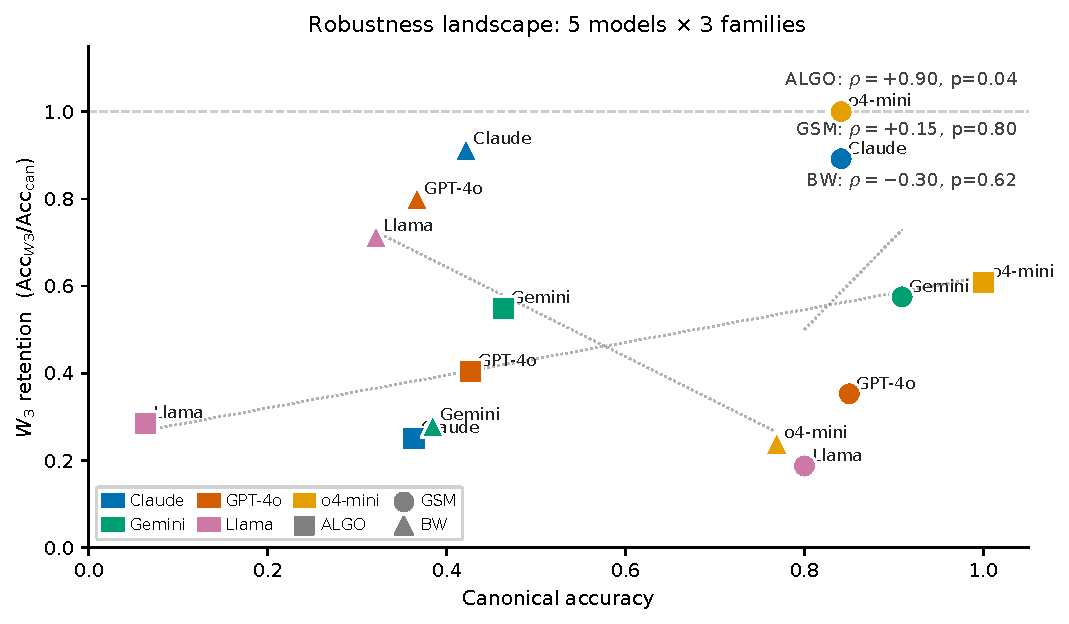
\includegraphics[width=\linewidth]{figures/fig_landscape.pdf}
  \caption{Accuracy--robustness landscape across five models and three
  families. Each point is one (model, family) pair. Within ALGO, more
  accurate models retain more of their canonical accuracy under \wthree{}
  ($\rho{=}{+}0.90$, $p{=}0.04$); the GSM trend is the same direction but
  n.s.\ ($\rho{=}{+}0.15$, $p{=}0.80$). On BW the rank-order is essentially
  flat ($\rho{=}{-}0.30$, $p{=}0.62$). \omini{} leads on GSM and ALGO
  retention but sits near the bottom on BW---a family-specific fragility
  invisible from absolute accuracy.}
  \label{fig:landscape}
\end{figure}

\begin{figure}[t]
  \centering
  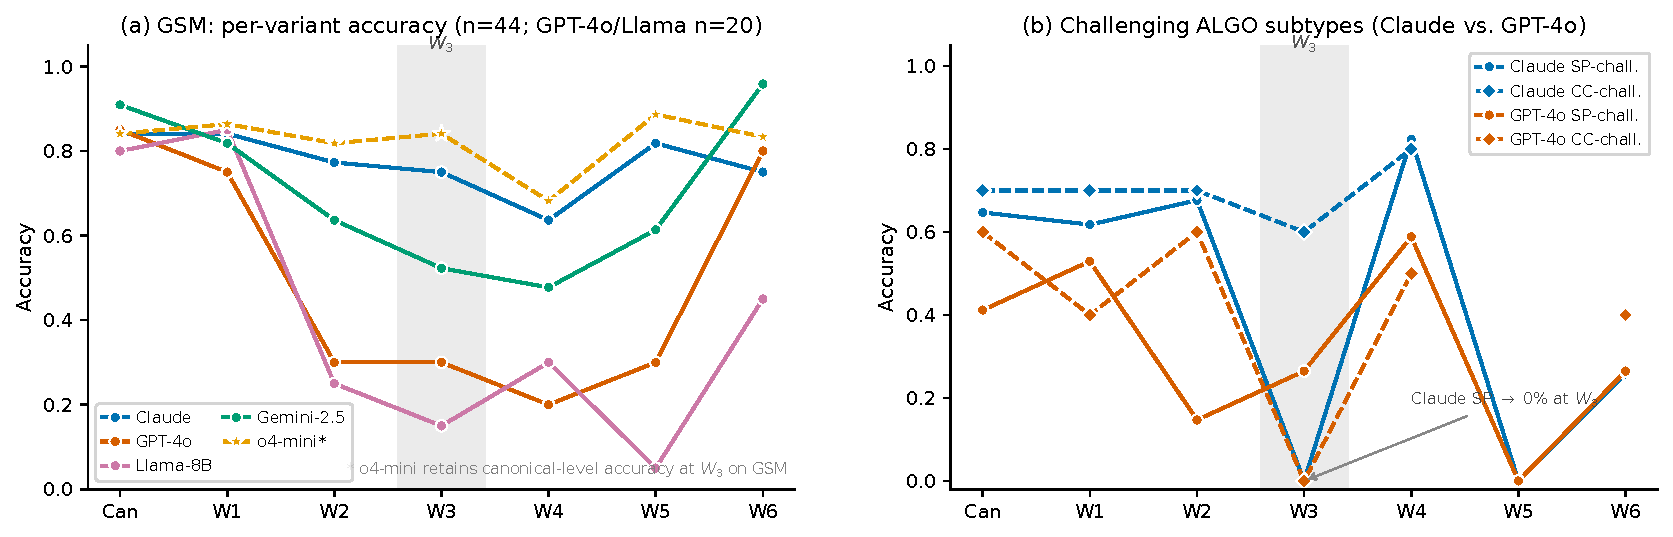
\includegraphics[width=\linewidth]{figures/fig_decay.pdf}
  \caption{Per-variant accuracy profiles (Probe~1). (a)~GSM: \wthree{} drops
  sharply for GPT-4o, Llama, and Gemini; for Claude it is mid-ranked. W6 (new
  numbers) stays much closer to canonical than \wthree{} for the
  higher-accuracy models. (b)~Challenging ALGO subtypes (Claude vs.\ GPT-4o):
  the dissociation at \wthree{} reverses between SP and CC.}
  \label{fig:pervariant}
\end{figure}

\begin{figure}[t]
  \centering
  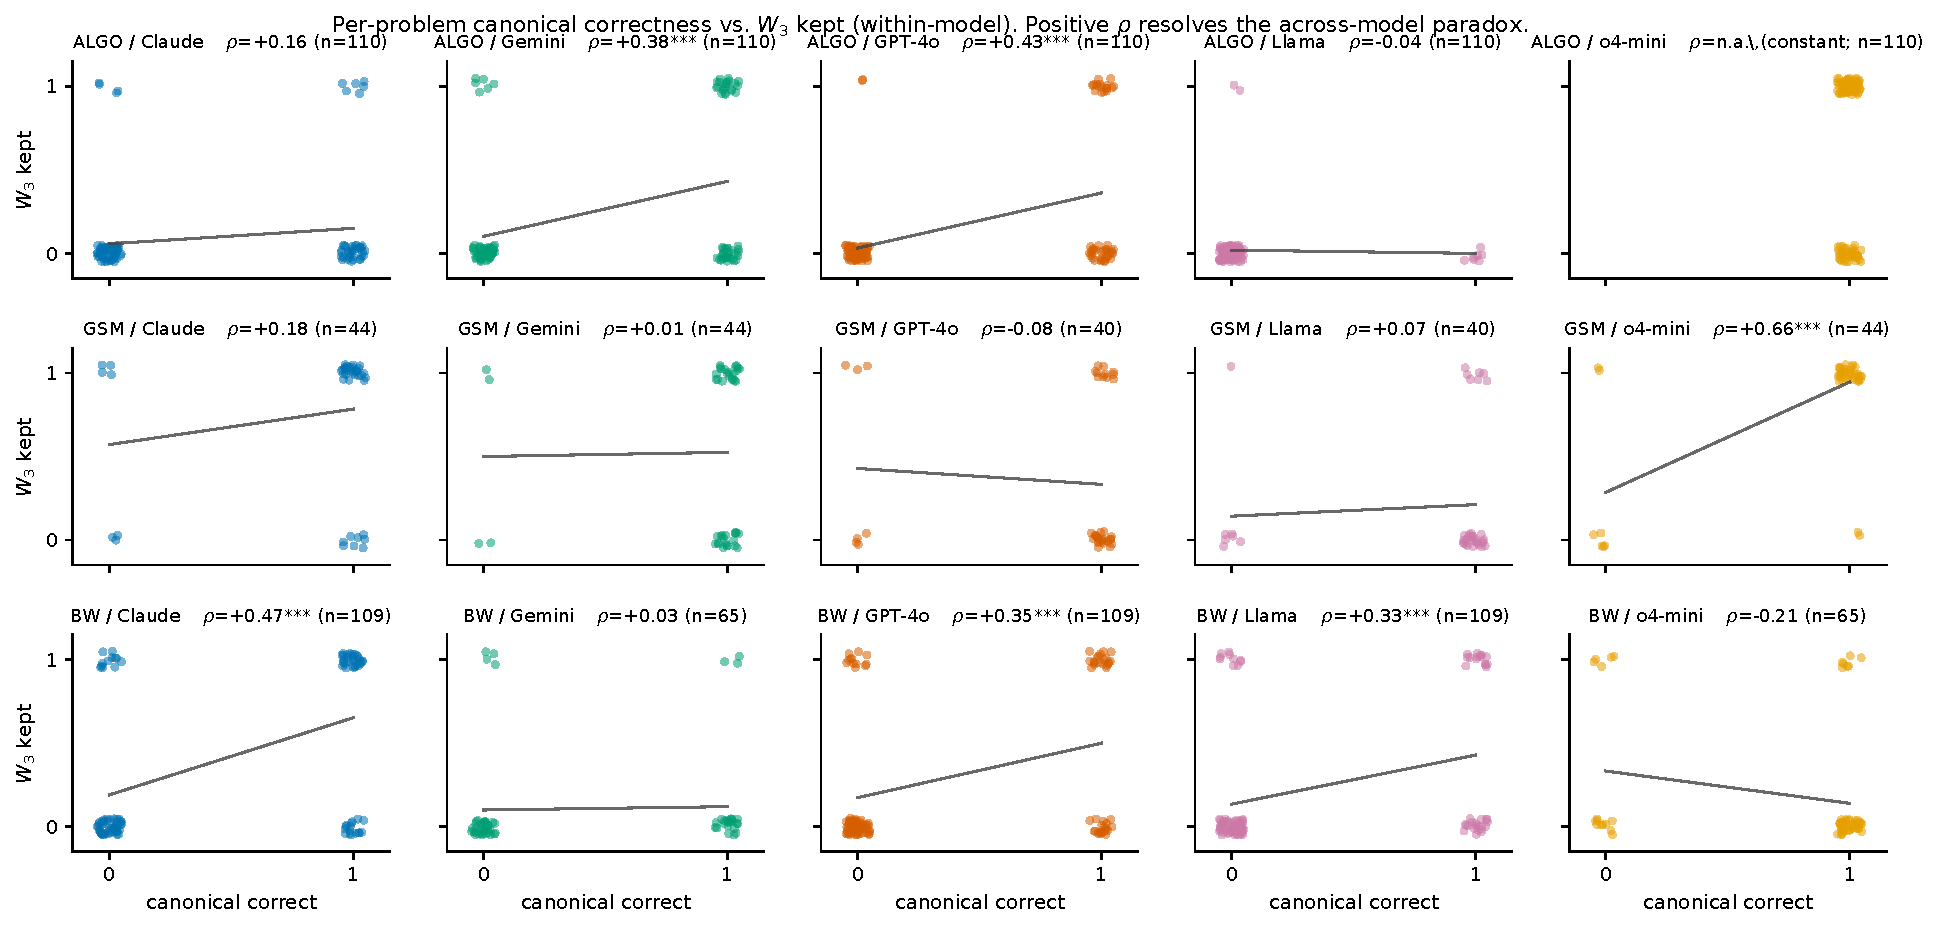
\includegraphics[width=\linewidth]{figures/fig_within_model.pdf}
  \caption{Within-model per-problem canonical correctness vs.\ \wthree{}
  correctness (3 families $\times$ 5 models). Each cell reports the Spearman
  $\rho$ between two binary indicators ($^{***}p{<}0.001$, $^{**}p{<}0.01$,
  $^{*}p{<}0.05$). Positive $\rho$ in most cells resolves the
  model-rank-level finding into a within-model rule: harder canonical
  problems also lose more under \wthree{}. Llama and \omini{} on BW are the
  only flat/negative cells.}
  \label{fig:within}
\end{figure}

\begin{figure}[t]
  \centering
  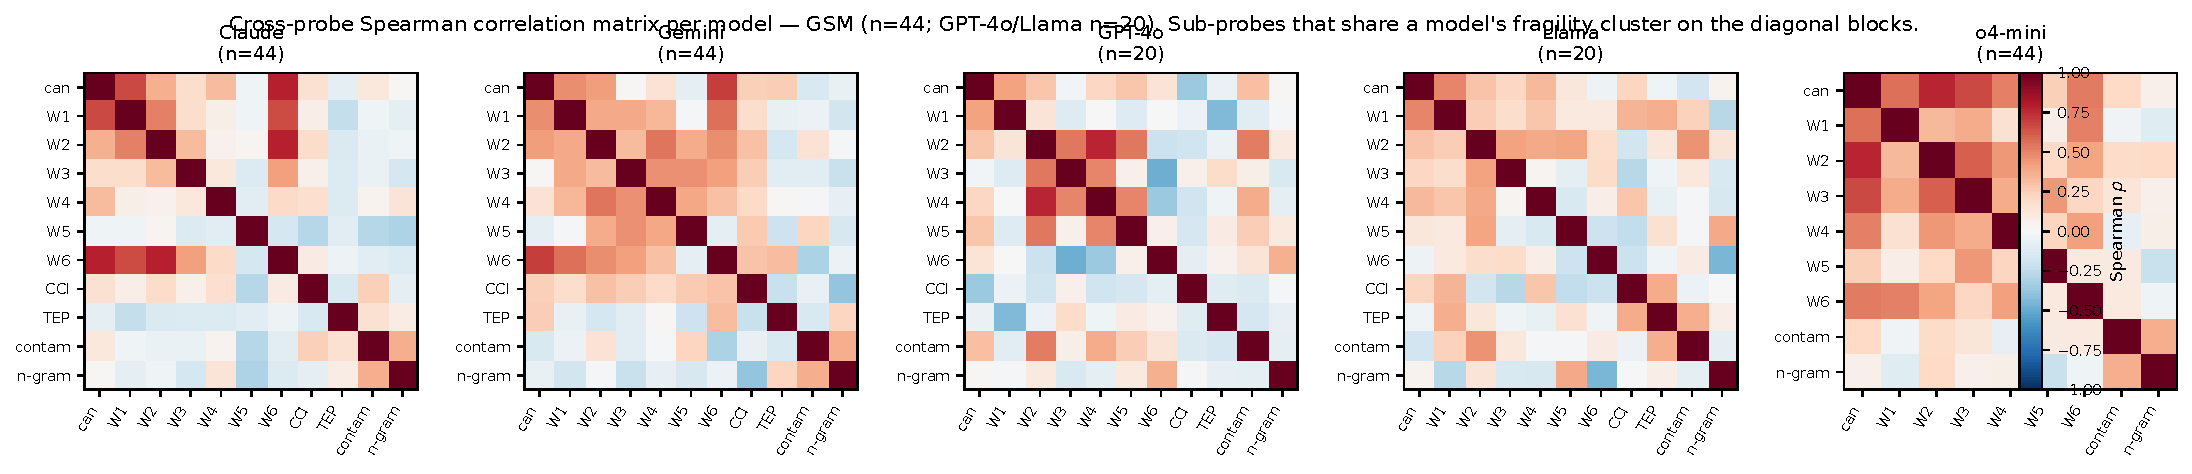
\includegraphics[width=\linewidth]{figures/fig_corr_matrix.pdf}
  \caption{(a)~GSM macro metrics: Gemini peaks on
  $\mathrm{Acc}_{\mathrm{can}}$ (0.91) and CCI (0.27) but only mid-pack on
  $\Rwiii$ (0.57); \omini{} reaches $\Rwiii{=}1.00$. (b)~Proximity
  predicts \vri{} for Claude ($r{=}{+}0.44^{***}$) and GPT-4o
  ($r{=}{+}0.37^{**}$) only; predicts CCI for Claude ($r{=}{+}0.31^{*}$).}
  \label{fig:macro}
\end{figure}

\begin{figure}[t]
  \centering
  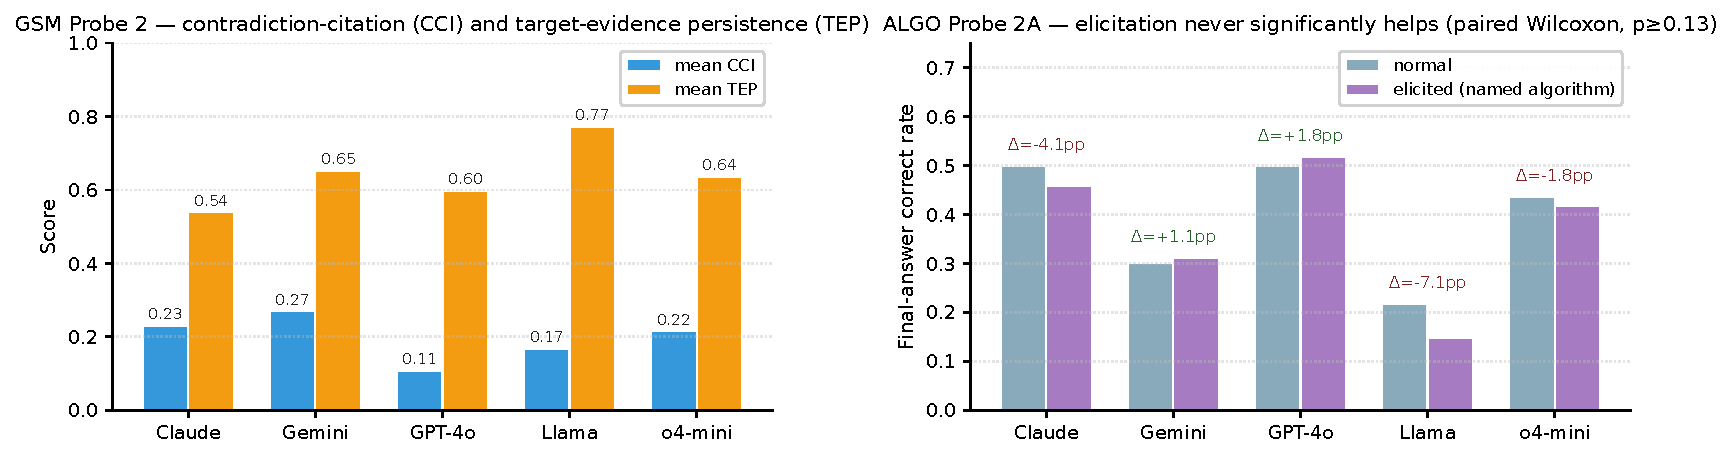
\includegraphics[width=\linewidth]{figures/fig_probe2_summary.pdf}
  \caption{Probe-2 summary across five models. \emph{Left:} GSM
  contradiction-citation index (CCI) and target-evidence persistence (TEP) per
  model on the full 44-problem GSM-P2 corpus. CCI rarely exceeds 0.30 for any
  model; TEP is high for every model (mean $\sim$0.6--0.8): the injected wrong
  value propagates through many subsequent steps, yet the final answer
  survives at near-baseline rates.
  \emph{Right:} ALGO Probe-2A final-answer accuracy with and without
  algorithm-elicitation; per-model deltas range from $-7.1$pp (Llama) to $+1.8$pp (GPT-4o), and the pooled paired Wilcoxon over $n{=}403$
  problem-instances is $p{=}0.20$. Elicitation never significantly improves
  final accuracy.}
  \label{fig:probe2summary}
\end{figure}

\begin{figure}[t]
  \centering
  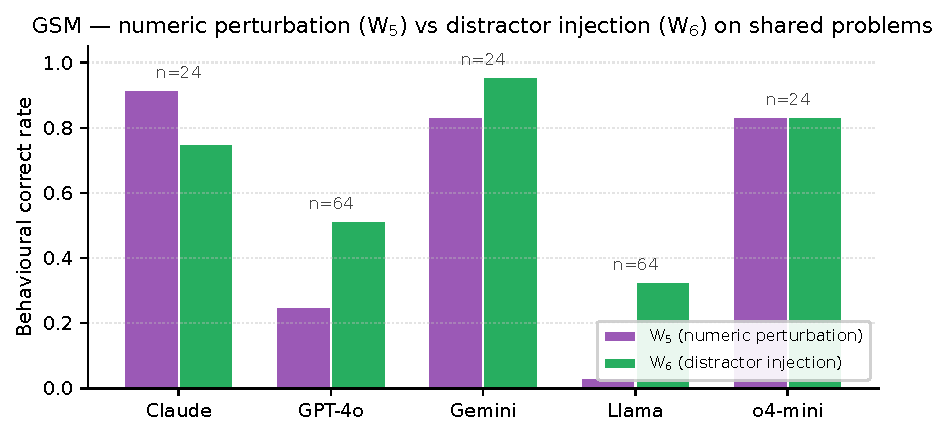
\includegraphics[width=\linewidth]{figures/fig_gsm_w5w6.pdf}
  \caption{GSM numeric perturbation (W5) vs.\ distractor injection (W6) on
  shared problems, per model. W6 (new numbers, same algorithm) stays close to
  canonical accuracy for the higher-accuracy models, while W5 (direction
  reversal) produces larger drops. Sample sizes vary by model due to the
  bank-valid subset constraint ($n{=}24$ for Claude/Gemini/\omini; $n{=}40$
  for GPT-4o/Llama).}
  \label{fig:gsmw5w6}
\end{figure}

\paragraph{BW subset note.}
BW Probe~1 accuracies are computed from \texttt{behavioral\_correct}
restricted to the $n{=}65$ question-bank IDs (50 standard Blocksworld + 15
Mystery Blocksworld), drawn from PlanBench~\citep{valmeekam2023planbench}. The
shipped raw file \texttt{BW\_P1\_behavioral.csv} additionally contains 44
PlanBench-extended instances; if those are included unfiltered, canonical
accuracies rise to 0.42 (Claude), 0.37 (GPT-4o), and 0.32 (Llama), because the
extra problems are markedly easier than the bank subset. We report the
bank-restricted numbers throughout for cross-family comparability.

\paragraph{GSM source files.}
GSM Probe-1 numbers in Tables~\ref{tab:gsm_p1} and~\ref{tab:pervariant} are
computed from the per-model raw files
(\texttt{GSM\_P1\_behavioral\_\{claude,gpt4o,llama,gemini,o4mini\}.csv}), with
$n{=}44$ for Claude/Gemini/\omini{} and $n{=}20$ for GPT-4o/Llama
(GSM\_001--020 only; GSM\_021--040 are off-bank duplicate reruns and
GSM\_041--064 are pending API gap fill, both excluded).

\paragraph{\omini{} scoring notes.}
\omini{} Blocksworld results in Table~\ref{tab:pervariant} ($n{=}65$ bank,
canonical .769) are computed from the NL-tolerant rerun; the original
PDDL-strict pass scored 0/65 because PDDL tuples do not match the NL grader
applied to other models. ALGO \omini{} accuracy is computed from the
per-instance verified column (canonical 110/110 on the full instance pool).

\begin{table}[t]
  \centering
  \small
  \setlength{\tabcolsep}{4pt}
  \caption{Per-variant accuracy by family, slice, and model (Probe~1). GSM
  uses rescored \texttt{included=True} rows; GPT-4o and Llama have $n{=}20$
  (bank-valid GSM\_001--020 only). ALGO uses the released verifier
  rescored offline (SP $W_3$ node mapping restored; trailing Path line
  preferred) on the frozen 61-ID challenging/standard split; \omini{} is
  omitted from ALGO rows. BW is bank-restricted to the $n{=}65$
  PlanBench IDs used throughout. ALGO and BW $W_6$ exclude byte-identical
  copies (25 ALGO WIS generator bug; 8 BW true duplicates). GSM $W_6$ is
  retained for models with bank rows (Claude/Gemini/\omini{} on GSM\_041--064).
  GPT-4o and Llama $W_6$ cells are omitted (\texttt{missing\_bank\_row}: Table~7
  .800/.450 were computed on GSM\_001--020 W6 in raw logs; no bank version
  ever defined W6 on those IDs). BW $W_5$
  drops MBW\_496--500 (identical to canonical; n=60). ALGO accuracies are
  still reported on the frozen 61-ID split of the 110 canonical IDs, but
  near-duplicate detection (normalized text + identical gold) collapses
  the 110-problem bank to effective $n{=}51$ (14 clone families covering
  73 problems); see \texttt{results/derived/bank\_clone\_audit.csv}.
  All remaining cells are the output of the released per-instance
  verifiers (Appendix~\ref{app:repro}).}
  \label{tab:pervariant}
  \begin{tabular}{lllccccccc}
    \toprule
    Family & Slice & Model & Can. & W1 & W2 & W3 & W4 & W5 & W6 \\
    \midrule
    GSM & -- & Claude     & .841 & .841 & .773 & .750 & .636 & .818 & .750 \\
    GSM & -- & GPT-4o     & .850 & .750 & .300 & .300 & .200 & .300 & --- \\
    GSM & -- & Gemini     & .909 & .818 & .636 & .523 & .477 & .614 & .958 \\
    GSM & -- & Llama      & .800 & .850 & .250 & .150 & .300 & .050 & --- \\
    GSM & -- & \omini     & .841 & .864 & .818 & .841 & .682 & .886 & .833 \\
    \midrule
    ALGO & CC-chall. & Claude     & .700 & .700 & .700 & .600 & .800 & --- & --- \\
    ALGO & CC-chall. & GPT-4o     & .600 & .400 & .600 & .600 & .500 & --- & --- \\
    ALGO & CC-chall. & Gemini     & .500 & .700 & .600 & .700 & .700 & --- & --- \\
    ALGO & CC-chall. & Llama      & .200 & .100 & .400 & .000 & .222 & --- & --- \\
    ALGO & CC-std. & Claude     & .267 & .467 & .067 & .300 & .667 & --- & .067 \\
    ALGO & CC-std. & GPT-4o     & .267 & .400 & .000 & .071 & .867 & --- & .200 \\
    ALGO & CC-std. & Gemini     & .267 & .133 & .000 & .000 & .267 & --- & .267 \\
    ALGO & CC-std. & Llama      & .000 & .067 & .111 & .000 & .000 & --- & .067 \\
    ALGO & SP-chall. & Claude     & .941 & .941 & .676 & .882 & .941 & .000 & .323 \\
    ALGO & SP-chall. & GPT-4o     & .412 & .529 & .147 & .294 & .676 & .000 & .258 \\
    ALGO & SP-chall. & Gemini     & .706 & .471 & .235 & .353 & .912 & .100 & .129 \\
    ALGO & SP-chall. & Llama      & .029 & .147 & .029 & .000 & .088 & .000 & .129 \\
    ALGO & SP-std. & Claude     & .952 & 1.000 & .762 & 1.000 & 1.000 & .053 & .579 \\
    ALGO & SP-std. & GPT-4o     & .762 & .667 & .048 & .476 & .714 & .000 & .368 \\
    ALGO & SP-std. & Gemini     & .619 & .762 & .810 & .476 & 1.000 & .083 & .333 \\
    ALGO & SP-std. & Llama      & .048 & .143 & .000 & .000 & .143 & .053 & .105 \\
    ALGO & WIS-chall. & Claude     & .353 & .176 & .118 & .000 & .067 & --- & --- \\
    ALGO & WIS-chall. & GPT-4o     & .353 & .176 & .000 & .000 & .000 & --- & --- \\
    ALGO & WIS-chall. & Gemini     & .353 & .176 & .000 & .000 & .000 & --- & --- \\
    ALGO & WIS-chall. & Llama      & .059 & .000 & .000 & .059 & .000 & --- & --- \\
    ALGO & WIS-std. & Claude     & .077 & .231 & .231 & .091 & .077 & --- & --- \\
    ALGO & WIS-std. & GPT-4o     & .154 & .231 & .000 & .000 & .000 & --- & --- \\
    ALGO & WIS-std. & Gemini     & .000 & .000 & .231 & .182 & .000 & --- & --- \\
    ALGO & WIS-std. & Llama      & .000 & .000 & .000 & .077 & .000 & --- & --- \\
    \midrule
    BW & -- & Claude     & .172 & .138 & .305 & .100 & .119 & .873 & .673 \\
    BW & -- & GPT-4o     & .063 & .172 & .102 & .100 & .119 & .291 & .250 \\
    BW & -- & Gemini     & .391 & .259 & .237 & .133 & .068 & .764 & .404 \\
    BW & -- & Llama      & .016 & .052 & .017 & .050 & .000 & .000 & .019 \\
    BW & -- & \omini     & .781 & .862 & .831 & .483 & .475 & .909 & 1.000 \\
    \bottomrule
  \end{tabular}
\end{table}


\paragraph{Population-level dissociation test.}
We test whether the pairwise inversions in Section~\ref{sec:inversion}
generalise to a population-level inverse relationship between canonical
accuracy and \wthree{} retention (Figure~\ref{fig:population}). At the
subtype$\times$model cell level, pooled across GSM, ALGO and BW: Spearman
$r{=}{+}0.147$ ($p{=}0.46$, $n{=}28$, 95\% bootstrap CI $[-0.27,+0.56]$);
ALGO-only $r{=}{+}0.37$ ($p{=}0.10$, $n{=}20$). At the per-problem level the
phi coefficients within each model are predominantly non-negative: ALGO
$\phi_{\text{Claude}}{=}{+}0.16$, $\phi_{\text{Gemini}}{=}{+}0.38$,
$\phi_{\text{GPT-4o}}{=}{+}0.43$, $\phi_{\text{Llama}}{=}{-}0.04$; GSM
$\phi_{\text{GPT-4o}}{=}{-}0.03$ ($n{=}20$ bank-valid),
$\phi_{\text{\omini}}{=}{+}0.66$; BW $\phi_{\text{Claude}}{=}{+}0.47$,
$\phi_{\text{GPT-4o}}{=}{+}0.35$, $\phi_{\text{Llama}}{=}{+}0.33$. The only
clearly negative cells are Llama on ALGO and \omini{} on BW. The aggregate
Spearman is indistinguishable from zero, so the pairwise inversions are real
per-(model, subtype) phenomena, not a universal inverse axis.

\begin{figure}[t]
  \centering
  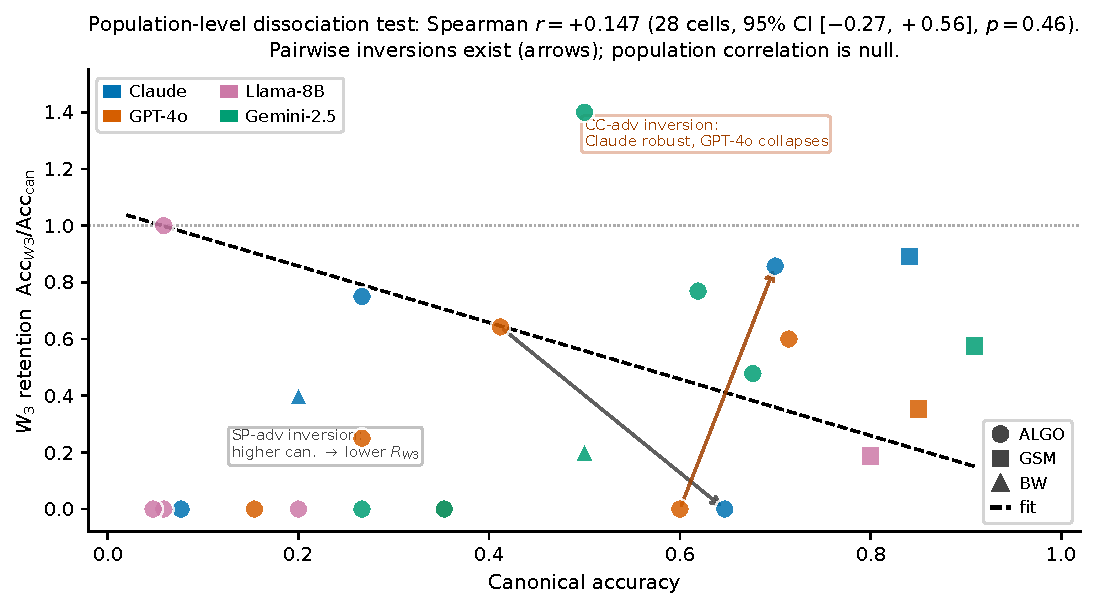
\includegraphics[width=\linewidth]{figures/fig_population.pdf}
  \caption{Population-level dissociation test. Each point is one (model,
  family/subtype, instance-type) cell. The two matched-canonical inversion
  pairs that drive the headline finding (SP-adv and CC-adv,
  Claude$\leftrightarrow$GPT-4o) are highlighted. Pooled Spearman is positive
  but indistinguishable from zero, so the dissociation is genuinely
  per-(model, subtype), not a universal axis.}
  \label{fig:population}
\end{figure}

\begin{figure}[t]
  \centering
  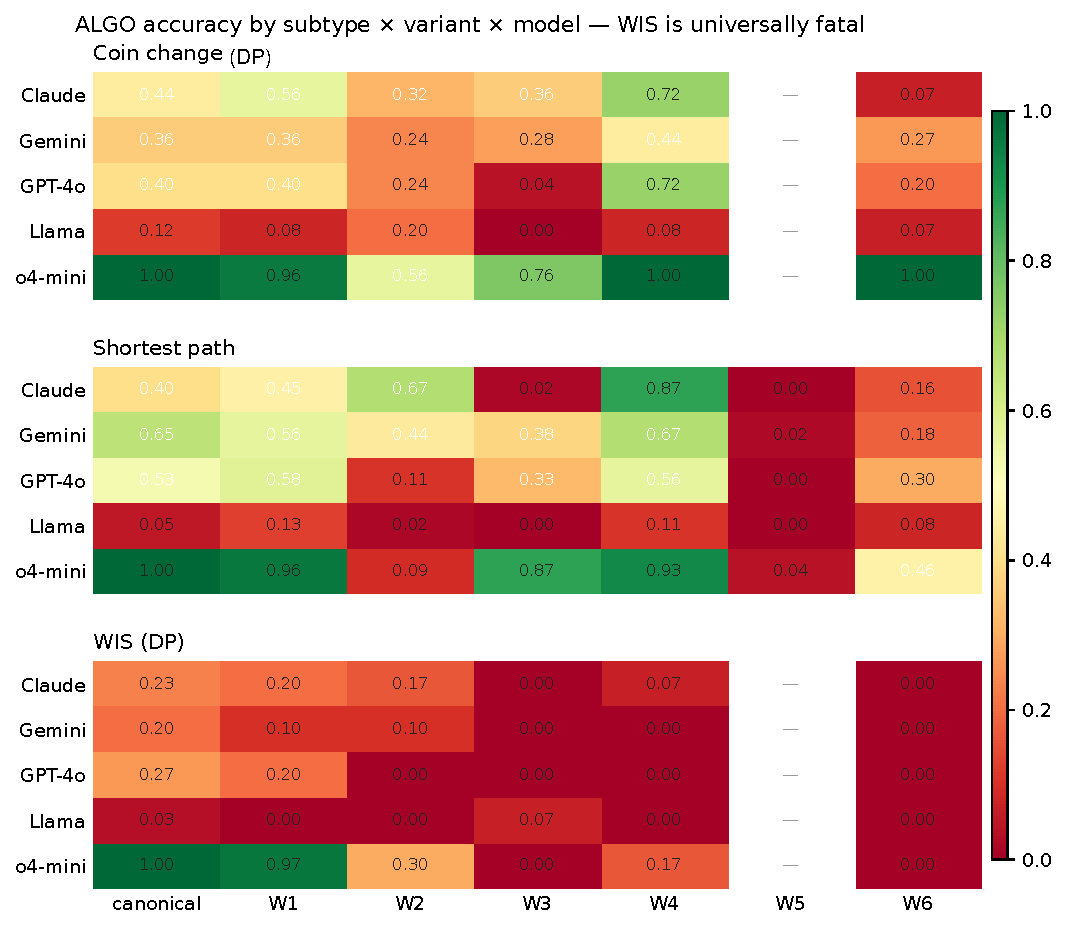
\includegraphics[width=\linewidth]{figures/fig_subtype_grid.pdf}
  \caption{ALGO accuracy decomposed by subtype $\times$ variant $\times$ model
  (3 subtypes $\times$ 7 variants $\times$ 5 models). The WIS row is the
  universal Achilles heel of every model; shortest-path W5 is a hard floor
  across the suite; coin change (CC) is the only subtype where renaming
  retention is non-trivial. (Note: CC is a dynamic-programming problem; the
  point of the subtype is precisely that a greedy heuristic is \emph{not}
  optimal for the general coin systems used here.) \omini's perfect canonical
  row does not carry to W3/W6 on WIS, isolating algorithmic depth as a
  distinct robustness axis.}
  \label{fig:algo_grid}
\end{figure}

% =====================================================================
\section{Probe 2 Protocol Details}
\label{app:probe2}

\paragraph{GSM Probe 2.}
\emph{Phase 1 (Declaration).} The model produces a complete step-by-step
solution with an explicit intermediate numeric value at each step (step
index, operation, numeric output). \emph{Phase 2A (Normal execution).} A
fresh API session per step; the model receives the original problem, step
index, and minimal state---no Phase-1 plan and no chat history from earlier
Phase-2A steps. Each Phase-2A output is compared to the Phase-1 declared value
via $\mathrm{match}_i{=}\mathbf{1}[|v_i^{(1)}-v_i^{(2)}|\leq 0.01]$; CCI is the
mean. \emph{Phase 2B (Injection).} Identical to 2A up to a uniformly sampled
injection step (excluding the first and last 10\% of the trajectory); the true
intermediate value is replaced with a plausible-magnitude but incorrect value.
Subsequent steps are classified for TEP relative to the uninjected run.

\paragraph{ALGO Probe 2.}
\emph{Phase 1.} Four-field JSON prompt: (1) named algorithm and why; (2) will
greedy work, why/why not; (3) first decision from the initial state; (4) at
which step greedy is most likely to fail. \emph{Phase 2A.} Fresh session per
step with problem, current state, and minimal step context (no prior chat
history); 30-step budget. \emph{Phase 2B.} As 2A, except the injection step
replaces the true state with one frontier-cost modification (SP), one
interval-boundary modification (WIS), or one coin-denomination addition (CC),
designed to be locally plausible but globally incorrect if propagated.

\paragraph{Plausible/implausible-injection aggregate gap.}
In the post-injection arm, the aggregate ``implausible'' condition has a
higher correct rate (54.1\%, $n{=}122$) than ``plausible'' (39.3\%,
$n{=}244$; Fisher $p{=}0.010$). This aggregate gap is a sampling artifact: the
implausible arm contains only Claude and GPT-4o sessions, while the plausible
arm additionally contains Llama (22.9\%) and Gemini (31.1\%), which depress
the plausible mean. Within the two models tested on both arms, the difference
is 0pp for Claude (52.5\% in both) and ${+}4.9$pp for GPT-4o (50.8\% vs.\
55.7\%). We therefore draw no behavioral conclusion from the aggregate gap.

\paragraph{Reasoning-type classification.}
Each Phase-2A step is assigned one of five reasoning types---unclear,
local-greedy, forward-simulation, algorithm-invocation, or backtracking---by a
deterministic rule-based classifier that matches lexical and structural cues in
the step text (e.g.\ an explicit named algorithm such as ``Dijkstra'' or
``dynamic programming'' for algorithm-invocation; an explicit revision of a
prior decision for backtracking). The decision rules are listed in
Appendix~\ref{app:prompts}. Because the classifier is deterministic, its labels
are exactly reproducible from the released step logs; a complementary
LM-judge cross-check on a 100-step sample is a planned extension.

\paragraph{Blocksworld Probe 2.}
\emph{Phase 1.} The model declares a full sequence of PDDL (action object)
tuples. \emph{Phase 2A.} Each declared step is executed within a PDDL
state-transition simulator; legal actions advance the state, illegal actions
are recorded, and sessions abort after 15 consecutive illegal actions.
84--100\% of sessions abort before plan completion (Section~\ref{sec:bw}).

\begin{figure}[t]
  \centering
  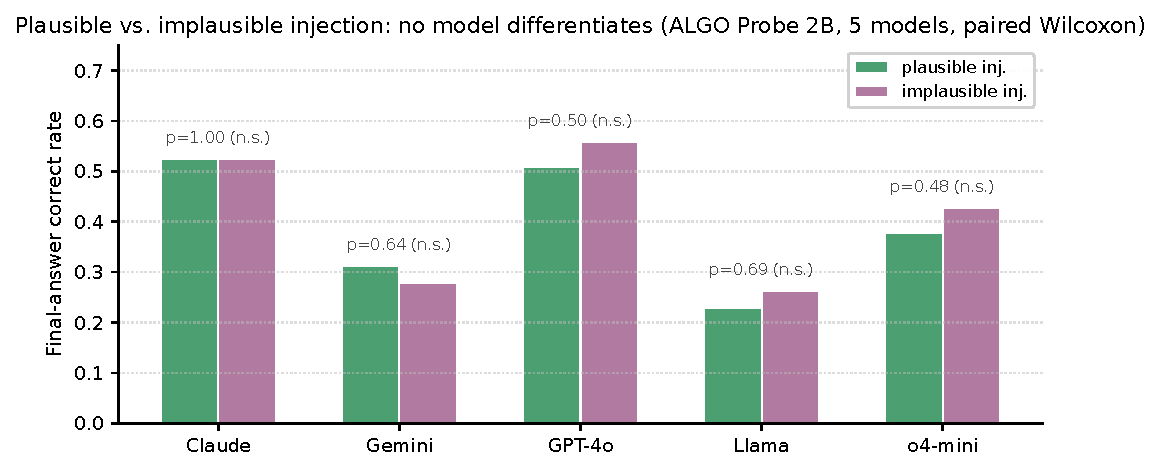
\includegraphics[width=\linewidth]{figures/fig_implaus.pdf}
  \caption{Plausible vs.\ implausible mid-stream injection, ALGO Probe~2B,
  $n{=}61$ paired problems per model. Paired-Wilcoxon $p$-values shown above
  each pair; no model differentiates the two arms.}
  \label{fig:plausible}
\end{figure}

\begin{figure}[t]
  \centering
  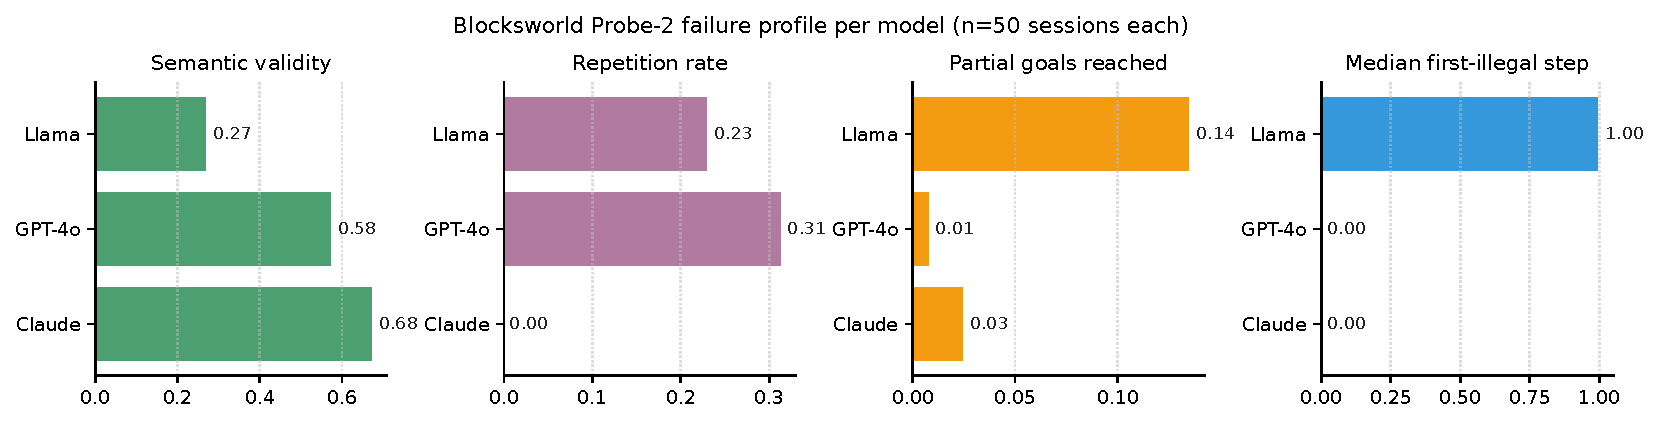
\includegraphics[width=\linewidth]{figures/fig_violations.pdf}
  \caption{Blocksworld Probe-2 failure profile per model ($n{=}50$ sessions
  each). Claude, GPT-4o, and Llama reach near-identical low CCI through three
  distinct breakdown modes: parse-formattable but semantically valid plans
  (Claude), high format errors with retained semantic validity (GPT-4o), and
  broad collapse plus heavy action repetition (Llama).}
  \label{fig:bw_profile}
\end{figure}

\begin{figure}[t]
  \centering
  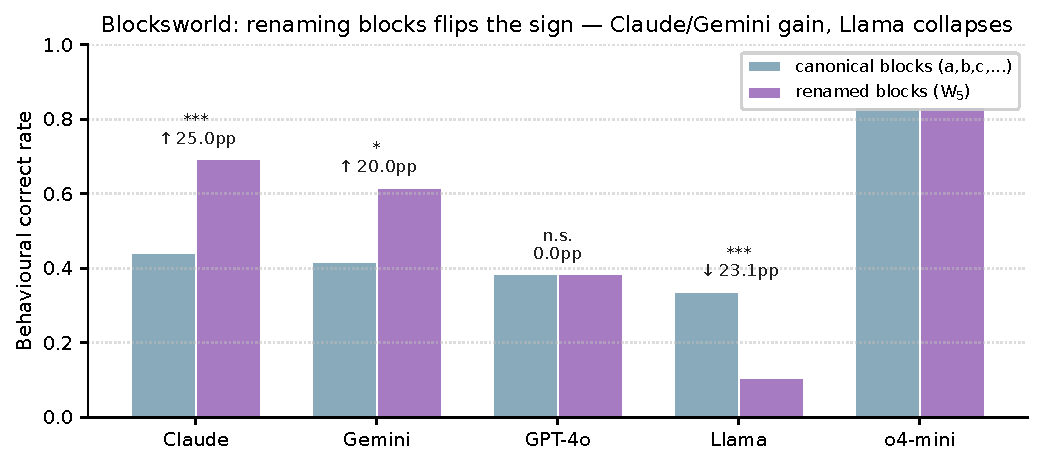
\includegraphics[width=\linewidth]{figures/fig_bw_inversion.pdf}
  \caption{Blocksworld canonical vs.\ renamed-blocks (W5) accuracy, per-model
  paired Wilcoxon. Renaming the canonical a,b,c,\ldots\ block tokens
  \emph{improves} Claude/Gemini (removes harmful retrieval cues),
  \emph{destroys} Llama (removes load-bearing cues), and leaves
  GPT-4o/\omini{} effectively untouched. The opposite signs across
  architectures are not consistent with a single mechanism.}
  \label{fig:bw_rename}
\end{figure}

% =====================================================================
\section{Mechanistic Rank Dissociation (Qwen pilot)}
\label{app:mech}

\paragraph{Why we ran a mechanistic check.}
A behavioural \wthree{} collapse alone cannot distinguish ``model genuinely
recomputes but fails surface mapping'' from ``model surfaces a memorised
canonical answer that no longer matches the renamed problem.'' The two
read-outs are confounded behaviourally but make opposite predictions inside
the residual stream of an open-weight model: under retrieval-style
commitment, the canonical gold token should remain highly accessible at the
final layer even though the problem has been renumbered; under recomputation,
those signatures should shift toward the variant's gold token. We run an
open-weight pilot on Qwen-2.5-7B~\citep{qwen2025technical} (28 transformer
layers), reading out four mechanistic signatures of the canonical gold token
per (problem family, variant): (1)~terminal commitment (median final-layer
rank); (2)~depth-resolved rank trajectory; (3)~depth-resolved calibrated
confidence ($\log p(\text{gold}\mid\text{prompt})$); and
(4)~depth-resolved representational alignment (cosine similarity to the gold
unembedding direction). Llama-3.1-8B~\citep{dubey2024llama} is the priority
follow-up.

\begin{figure}[t]
  \centering
  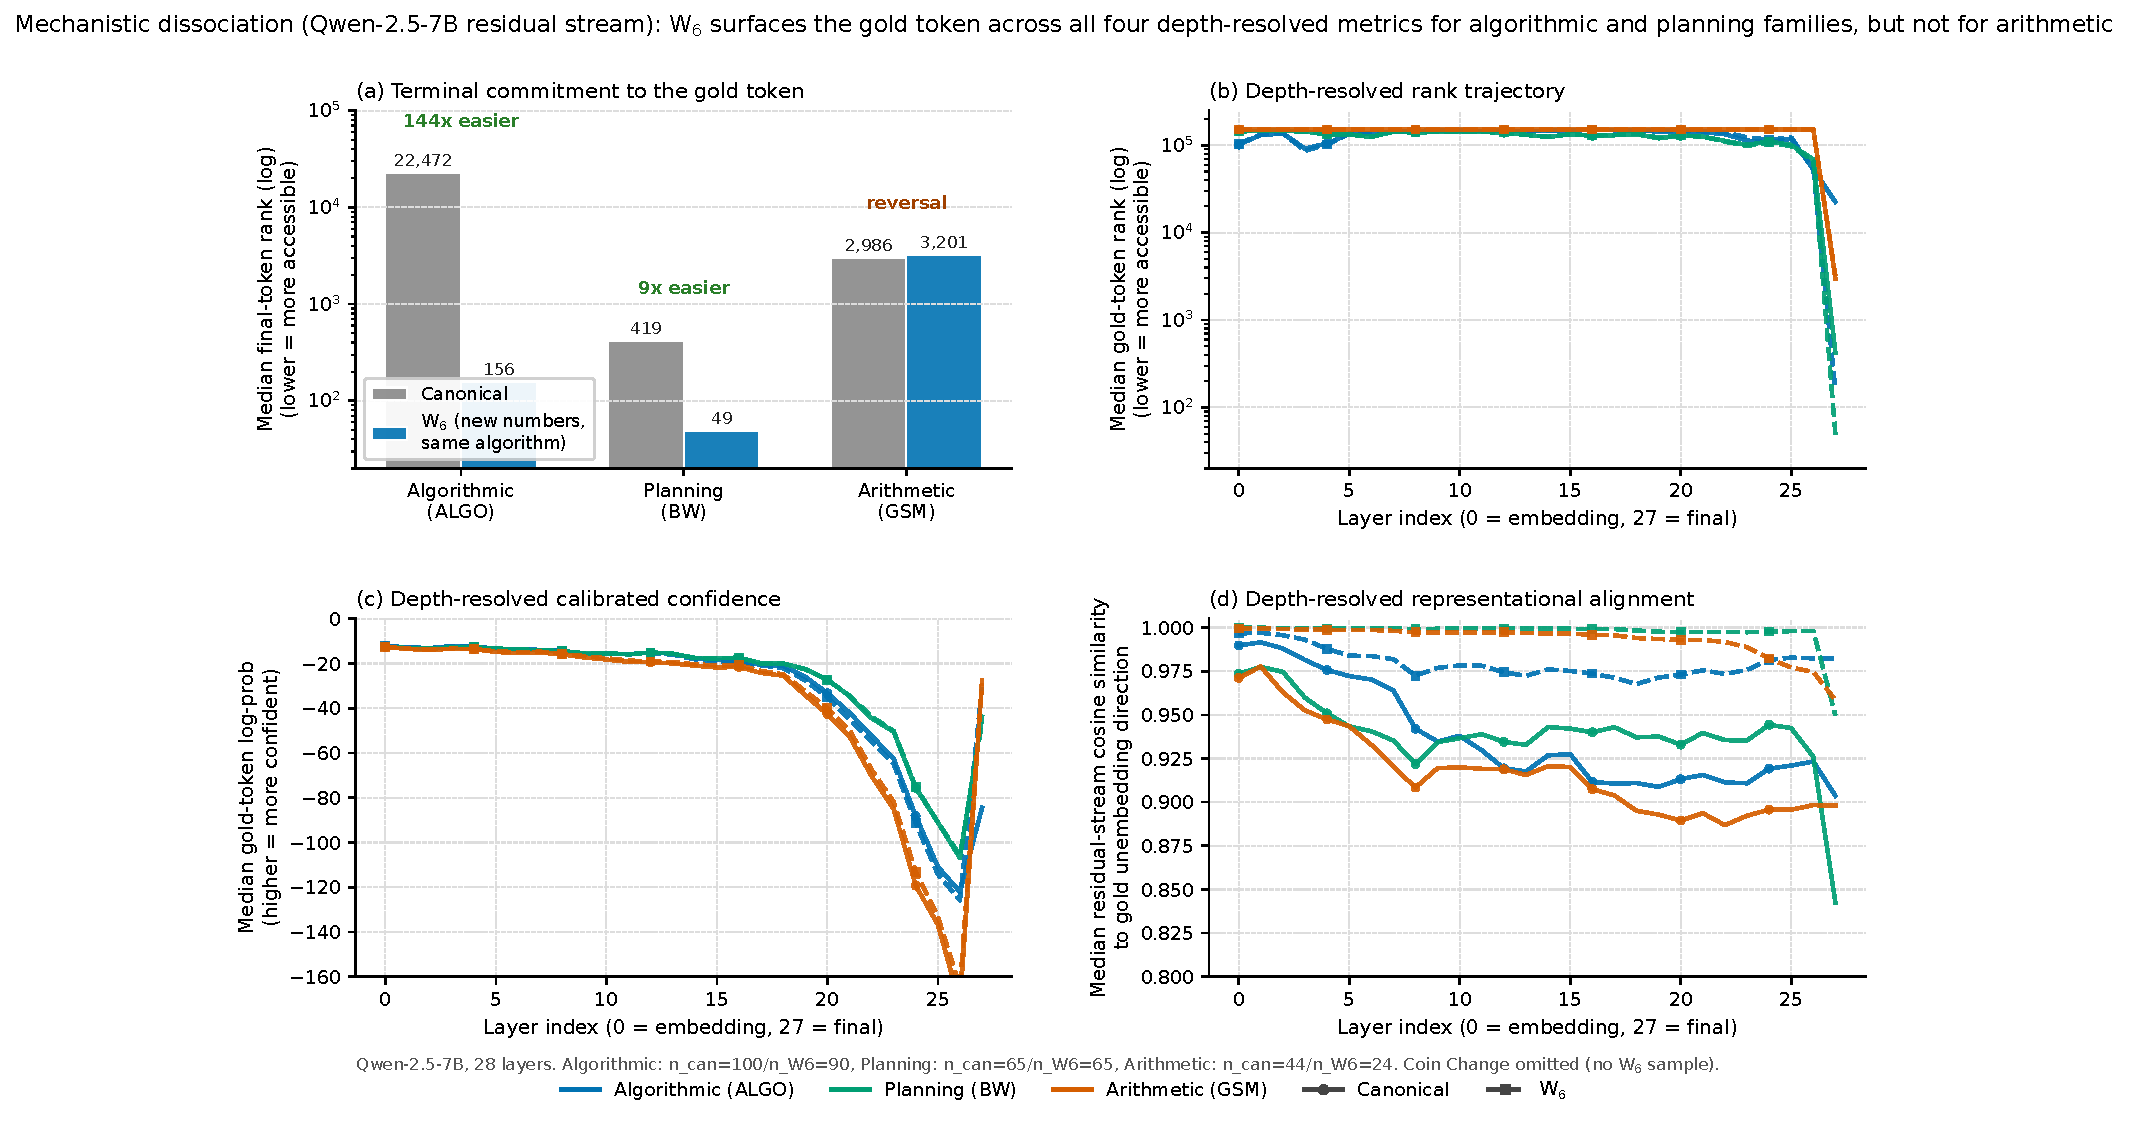
\includegraphics[width=\linewidth]{figures/fig_mechanistic.pdf}
  \caption{Mechanistic dissociation in the Qwen-2.5-7B residual stream,
  canonical vs.\ W6 (new numbers, same algorithm), across three families.
  (a)~Median final-token rank of the gold answer (log $y$-axis, lower is more
  accessible). (b)--(d)~Layer-by-layer median trajectories of gold-token rank,
  log-probability, and residual-stream cosine similarity. Algorithmic and
  planning families show the predicted dissociation on all four metrics; the
  arithmetic family does not (the final-layer rank moves in the opposite
  direction), so the mechanistic claim is scoped to algorithmic and planning,
  not arithmetic.}
  \label{fig:mechanistic}
\end{figure}

\paragraph{What the four metrics show.}
\emph{Terminal commitment.} Algorithmic: canonical median rank
22{,}472 collapses to 156 under W6 ($n_{\mathrm{can}}{=}100$,
$n_{W_6}{=}90$; $\sim$$144\times$ more accessible). Planning:
$419{\to}49$ ($n{=}65$; $\sim$$9\times$). Arithmetic: $2{,}985{\to}3{,}201$
($n{=}44/24$; a reversal). \emph{Depth-resolved rank.} For algorithmic and
planning, canonical and W6 trajectories are indistinguishable through layer
$\sim$24 then split sharply in the last 3--4 layers; for arithmetic both
collapse together. \emph{Log-prob} and \emph{cosine similarity} show the same
dissociation, with W6 keeping the residual stream closer to the gold direction
from layer $\sim$5 onward.

\paragraph{Paired statistics on aligned pairs.}
One-sided Wilcoxon (H1: canonical rank $>$ W6 rank): planning $n{=}65$,
median $\log_{10}(\text{can}/W_6){=}0.80$, $W{=}1359$,
$p{=}2.4{\times}10^{-6}$; algorithmic $n{=}90$, median ${=}0.00$, $W{=}1072$,
$p{=}0.079$ (borderline); arithmetic $n{=}24$, median ${=}{-}0.39$,
$p{=}0.63$ (reversal confirmed). The ``W6 surfaces gold token'' claim is
statistically robust for planning, directional but not population-significant
for algorithmic, and reversed for arithmetic.

\paragraph{The four metrics are not redundant.}
Final-token rank and log-probability correlate strongly ($r{=}{-}0.79$), but
final rank and final cosine similarity correlate only weakly
($r{=}{-}0.17$, $p{<}10^{-3}$) and final log-probability and final cosine
similarity are statistically independent ($r{=}{+}0.005$, n.s.). We present
all four because each isolates a distinct aspect of representational
alignment.

\paragraph{Scope and limitations.}
This is a single open-weight backbone; we do not claim the same per-layer
dynamics hold for frontier closed-weight models. The mechanistic result is
supportive of the behavioural pattern, not an explanation of it.

% =====================================================================
\section{Evaluation Pipeline Design}
\label{app:pipeline}

\paragraph{Data flow.} Four sequential stages: (1)~\textbf{Canonical problem
bank.} GSM: stratified sample from GSM8K~\citep{cobbe2021training} across four
Infini-gram contamination quartiles. ALGO: hand-designed CC/SP/WIS instances
with verified DP-optimal solutions. BW: instances from
PlanBench~\citep{valmeekam2023planbench}. (2)~\textbf{Variant generation.}
Each canonical problem expanded to 6 variants by deterministic scripts; every
variant passed through a domain verifier before storage. (3)~\textbf{Model
sweep.} All (problem, variant, model) triples queued via OpenRouter at
$T{=}0$, zero-shot CoT; Phase-2 probes run in strict session isolation.
(4)~\textbf{Verification and scoring.} Family-specific verifiers; per-instance
outputs written to raw CSVs that are the single source of truth.

\begin{figure}[h!]
  \centering
  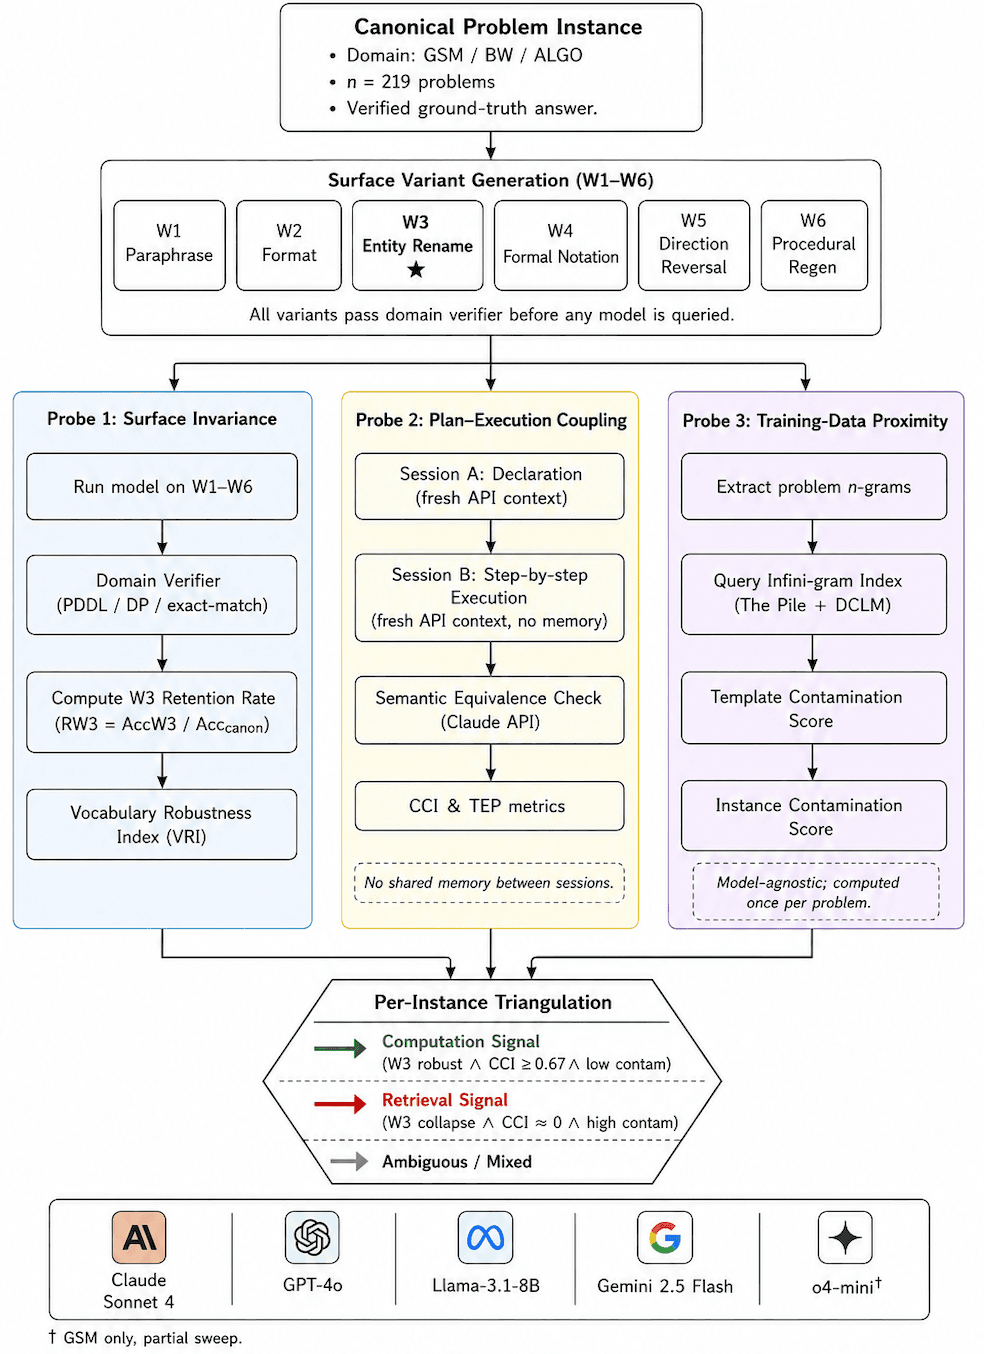
\includegraphics[width=\linewidth]{figures/pipeline.png}
  \caption{End-to-end pipeline. Each canonical problem generates six surface
  variants (W1--W6); Probe~1 records per-variant accuracy; Probe~2 spans three
  phases (declaration, execution, injection); Probe~3 queries the Infini-gram
  public-corpus index. All five models (Claude Sonnet~4, GPT-4o,
  Llama-3.1-8B, Gemini~2.5 Flash, \omini) are evaluated on every probe; the
  per-(probe, model) coverage matrix with intentional-scoping cells is in
  Table~\ref{tab:coverage_full}.}
  \label{fig:pipeline}
\end{figure}

% =====================================================================
\section{Reproducibility and Verification}
\label{app:repro}

All code, per-instance verifier logs, and variant generation templates are at
\url{https://anonymous.4open.science/r/retrieval-vs-computation-EA8F/README.md}
and will be moved to a permanent home upon acceptance. The bundle ships raw
per-instance verifier logs with a re-derivation script that recomputes every
aggregate cited in the main paper directly from those logs; the script applies
the bank-ID filter so GSM GPT-4o/Llama figures reproduce at $n{=}20$.
Reviewers can verify reported numbers without retraining or re-querying any
model. The repository contains no author-identifying information.
\textbf{Wilcoxon sensitivity.} Full bank $n{=}44$ (zero-imputed): $W{=}396$,
$p{=}0.0068$; paired $t{=}2.63$, $p{=}0.0072$. Complete-case analysis yields
the same $p$-values.

% =====================================================================
\section{Algorithm-Invocation Observation (Exploratory)}
\label{app:invocation}

Thirteen Phase-2 steps across Claude (6), Llama (4), and Gemini (3) were
classified as \emph{algorithm-invocation}: the model explicitly named a
specific algorithm (``I will use Dijkstra's algorithm'') and attempted to
apply it. All 13 yielded incorrect final answers
(Figure~\ref{fig:invocation}). Wilson 95\% CI on 0/13: $[0\%, 22.8\%]$.
Fisher's exact vs.\ unclear-reasoning baseline (138/1{,}041${=}13.3\%$):
$p{=}0.40$. This is an observational pattern with $n{=}13$, not a statistical
claim. Supporting observations: (a)~distributed across three of four models
(GPT-4o produced zero algorithm-invocation steps across the entire ALGO
sweep); (b)~selection effect ruled out (the 12 unique problems with
algorithm-invocation steps have \emph{higher} mean canonical accuracy, 0.292,
than the full ALGO set, 0.239; $t{=}0.81$, $p{=}0.42$); (c)~consistent
qualitative pattern (the model named the correct algorithm, then executed a
heuristic inconsistent with it). Table~\ref{tab:invocation} lists 10 of the 13
documented cases (3 Gemini cases omitted for space).

\begin{figure}[h!]
  \centering
  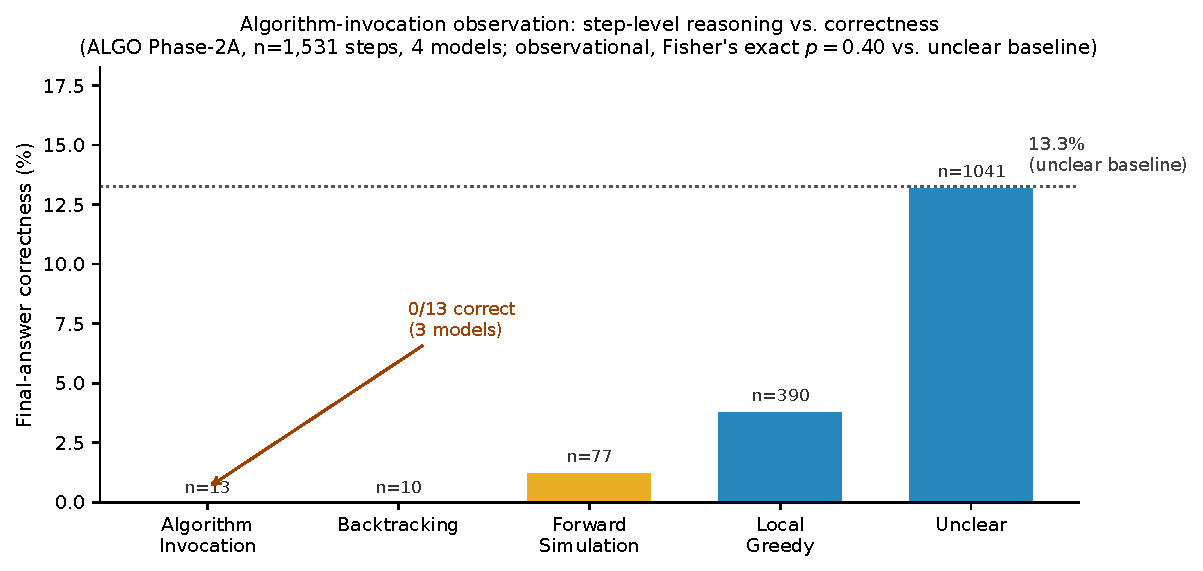
\includegraphics[width=\linewidth]{figures/fig_paradox.pdf}
  \caption{Step-level reasoning type vs.\ final-answer correctness across ALGO
  Phase-2A steps (4 models). Algorithm-invocation ($n{=}13$ steps, three models;
  $n{=}12$ unique problems---one problem contributed two invocation steps)
  yields 0\% correct final answers. Dotted line shows the unclear-reasoning
  baseline (13.3\%). Fisher's exact: $p{=}0.40$---not significant. This is an
  observational pattern, not a statistical claim.}
  \label{fig:invocation}
\end{figure}

\begin{table}[t]
  \centering
  \small
  \caption{Algorithm-invocation cases (10 of 13; 3 Gemini cases omitted for
  space). All yielded incorrect final answers; in every case Phase-2A
  execution reverted to a greedy heuristic after naming the algorithm.}
  \label{tab:invocation}
  \begin{tabular}{llll}
    \toprule
    Case & Problem & Slice & Model \\
    \midrule
    A1 & SP\_002  & SP-std   & Llama  \\
    A2 & SP\_004  & SP-chall & Claude \\
    A3 & SP\_037  & SP-chall & Claude \\
    A4 & SP\_040  & SP-chall & Claude \\
    A5 & SP\_044  & SP-chall & Llama  \\
    A6 & SP\_062  & SP-chall & Claude \\
    A7 & SP\_065  & SP-chall & Claude \\
    A8 & WIS\_003 & WIS-chall& Llama  \\
    A9 & WIS\_007 & WIS-std  & Llama  \\
    A10& WIS\_020 & WIS-chall& Claude \\
    \bottomrule
  \end{tabular}
\end{table}


% =====================================================================
\section{Triangulation Convergence Detail}
\label{app:triangulation}

ALGO (440 instances ${=}$ 110 problems $\times$ 4 models; \omini{} excluded
from strict triangulation because its constant W3${=}1.00$ on this family
makes the retrieval-vs-computation label degenerate): retrieval signal
${=}8$; computation signal ${=}4$; mixed ${=}157$; ambiguous ${=}271$
(61.6\%). GSM (Claude, $n{=}44$): converging-computation ${=}35$; diverging
${=}9$. BW (Claude, 124 instances including variants):
converging-computation ${=}4$; diverging ${=}41$; execution-unavailable
${=}25$; insufficient ${=}54$. Label rules: W3 at 0 or 1; CCI $\leq 0.10$ or
$\geq 0.67$; contamination at floor or above the 75th percentile.

\begin{table}[t]
  \centering
  \small
  \caption{Triangulation label rates on 440 ALGO instances under strict vs.\
  liberal threshold configurations. The strong-label rate is a design choice,
  not a fixed property of the data.}
  \label{tab:thresholds}
  \begin{tabular}{lcccc}
    \toprule
    Configuration & Retrieval & Computation & Strong total & Ambiguous \\
    \midrule
    Legacy strict (paper default) & 1.8\%  & 0.9\%  & 2.7\%  & 61.6\% \\
    Liberal v2 sweep (param 204)  & 27.3\% & 30.4\% & 57.7\% & 37.9\% \\
    \bottomrule
  \end{tabular}
\end{table}


% =====================================================================
\section{Prompts}
\label{app:prompts}

\textbf{Probe 1 (canonical and variants, all families).}\\
\texttt{Solve the following problem exactly and provide only the final answer
in the required output format. Problem: \{problem\}. Format instruction:
\{family\_specific\_output\_format\}.} The same template is used for canonical
and W1--W6; only \texttt{\{problem\}} changes.

\textbf{ALGO Phase 1 (declaration).}\\
\texttt{You are given the following problem: \{problem\}. Before solving it,
answer four structured questions: (1) Which named algorithm will you use, and
why is it appropriate? (2) Would a greedy approach work? Why or why not? (3)
What is your first decision from the initial state? (4) At which step is the
greedy approach most likely to fail? Respond with a JSON object using exactly
these keys: \{algorithm, greedy\_works, first\_move, critical\_step\}.}

\textbf{ALGO Phase 2A (step execution).}\\
\texttt{You are solving the following problem: \{problem\}. Current state:
\{state\}. Your prior decisions: \{trajectory\}. What is your next decision?
Provide a brief justification (1{-}2 sentences).}

\textbf{GSM Phase 1 (numeric plan declaration).}\\
\texttt{Solve the following arithmetic problem step by step. Before computing
each step, state what you will compute and why. After each step, write the
intermediate numeric result explicitly on its own line in the format: Step N
result: [value]. Problem: \{problem\}.}

\textbf{Reasoning-type classification (deterministic rules).} Each Phase-2A
step is assigned exactly one category by a rule-based classifier over the step
text, with the following decision criteria (evaluated in order; default
\texttt{unclear}):
\begin{itemize}
  \item \texttt{algorithm\_invocation} --- the step names a specific algorithm
  (e.g.\ ``Dijkstra'', ``dynamic programming'', ``knapsack'') and attempts to
  apply it.
  \item \texttt{backtracking} --- the step explicitly revises or undoes a prior
  decision.
  \item \texttt{forward\_simulation} --- the step explicitly considers future
  states or look-ahead paths.
  \item \texttt{local\_greedy} --- the step selects the option with the lowest
  immediate cost without considering future states.
  \item \texttt{unclear} --- none of the above cues are present.
\end{itemize}

\textbf{Probe 3 (training-data proximity query template).}\\
\texttt{For each problem text, compute template-level and instance-level
$n$-gram overlap against indexed corpora (The Pile, DCLM) and return a
normalized score in [0,1] for each field.}

Verifier outputs use deterministic parsing and exact checks: numeric
exact-match (GSM), DP-optimal answer match (ALGO), and goal-state reachability
(BW; strict and NL-tolerant variants both reported).

% =====================================================================
% Mandatory CAISc 2026 checklists. Rendered with the official style-file
% macros (\involvementA, \iterationLow, \answerYes, ...). Instruction
% blocks have been deleted per template; section/subsection headings and
% all questions are kept verbatim.
% =====================================================================

\newpage

\section*{Conference For AI Scientists 2026 - AI Involvement Checklist}
\label{checklist_ai_involvement}

\subsection*{Research Stage Assessment}

\begin{enumerate}

  \item \textbf{Hypothesis development}.

  Answer: \involvementA{}

  Iteration Effort: \iterationNA{}

  Explanation: The research problem, seed idea, and the three-probe
  triangulation framework were conceived and developed by the human authors.
  AI tools were not used to formulate the core research question or the
  framework design.

  \item \textbf{Experimental design and implementation}.

  Answer: \involvementB{}

  Iteration Effort: \iterationHigh{}

  Explanation: The experimental design, choice of baselines, problem families,
  and overall methodology were decided by the human authors. AI coding
  assistants implemented the experimental stack under human direction (the six
  variant-generation scripts, the five-model API sweep harnesses, the three
  family-specific verifiers, and the Infini-gram proximity pipeline) across
  many iterations of debugging and refinement. All design decisions, audit
  sign-off, and final code review were performed by the human authors.

  \item \textbf{Analysis of data and interpretation of results}.

  Answer: \involvementB{}

  Iteration Effort: \iterationMedium{}

  Explanation: Data processing and statistical analysis were primarily carried
  out by the human authors. AI tools assisted with data organisation and
  exploratory checks (for example, reconciling aggregate counts against the
  per-instance verifier logs and surfacing an off-bank duplicate-ID issue that
  the authors then excluded). All reported conclusions were drawn and verified
  by the human authors.

  \item \textbf{Writing}.

  Answer: \involvementB{}

  Iteration Effort: \iterationMedium{}

  Explanation: The manuscript was primarily written by the human authors. AI
  tools were used as writing aids for grammar, sentence restructuring, and
  clarity of exposition. All scientific content, arguments, and conclusions are
  the work of the human authors.

\end{enumerate}

\subsection*{AI System Documentation}

\begin{enumerate}
  \setcounter{enumi}{4}

  \item \textbf{AI systems used}.

  Description: A frontier large language model (accessed through a commercial
  chat interface and API) was used as a coding assistant, writing aid, and
  literature-review aid throughout the project, together with an AI-assisted
  integrated development environment for code completion and refactoring. A
  separate open-weight transformer language model (approximately 7B parameters)
  was the \emph{subject} of the mechanistic analysis in
  Appendix~\ref{app:mech}; it was not used as a research assistant. No custom
  multi-agent frameworks were used. Specific product and model names are
  withheld in this anonymized submission and will be disclosed in the
  camera-ready version.

  \item \textbf{Observed AI Limitations}.

  Description: Two limitations were observed. First, context inconsistency: AI
  coding assistance occasionally produced code subtly inconsistent with the
  existing pipeline (mismatched column names, off-by-one step indices, and in
  one case computing a GSM aggregate over off-bank duplicate problem IDs), each
  caught by human review before integration. Second, imprecise statistical
  language: AI-assisted writing drafts sometimes conflated correlation strength
  with statistical significance, which the human authors corrected before
  inclusion.

\end{enumerate}

\newpage

\section*{Conference For AI Scientists 2026 - Reproducibility and Responsibility Checklist}
\label{checklist_reproducibility}

\begin{enumerate}

\item {\bf Claims}
    \item[] Question: Do the main claims made in the abstract and introduction
    accurately reflect the paper's contributions and scope?
    \item[] Answer: \answerYes{}
    \item[] Justification: The abstract and introduction state three concrete
    findings (block-rename sign flip, WIS universal collapse, and
    injection-compliance/correctness dissociation), each supported in
    Sections~\ref{sec:inversion}--\ref{sec:bw} and~\ref{sec:conclusion} with
    explicit $n$, confidence intervals, and $p$-values. Scope is explicitly
    restricted to zero-shot structured reasoning.

\item {\bf Limitations}
    \item[] Question: Does the paper discuss the limitations of the work
    performed by the authors?
    \item[] Answer: \answerYes{}
    \item[] Justification: A dedicated Limitations section covers scope
    (English, zero-shot, structured reasoning), the Probe-3 proximity-proxy
    status, the Blocksworld measurement-protocol abort, single
    reasoning-trained provider, the behavioural-only scope of CCI, and deferred
    API-budget experiments. An explicit per-(probe, model) coverage matrix is
    given in Appendix~\ref{app:cov}.

\item {\bf Theory assumptions and proofs}
    \item[] Question: For each theoretical result, does the paper provide the
    full set of assumptions and a complete (and correct) proof?
    \item[] Answer: \answerNA{}
    \item[] Justification: The paper is empirical; it presents no formal
    theorems or proofs. All statistical methods and assumptions are documented
    in Appendix~\ref{app:metrics}.

\item {\bf Experimental result reproducibility}
    \item[] Question: Does the paper fully disclose all the information needed
    to reproduce the main experimental results?
    \item[] Answer: \answerYes{}
    \item[] Justification: All prompts and classifier rules are in
    Appendix~\ref{app:prompts}; all metric definitions in
    Appendix~\ref{app:metrics}; all model, temperature, and API settings in
    Section~\ref{sec:setup}. Per-instance verifier logs and a re-derivation
    script (which applies the bank-ID filter so the GSM GPT-4o/Llama figures
    reproduce at $n{=}20$) are shipped in the anonymous repository
    (Appendix~\ref{app:repro}).

\item {\bf Open access to data and code}
    \item[] Question: Does the paper provide open access to the data and code,
    with sufficient instructions to faithfully reproduce the main results?
    \item[] Answer: \answerYes{}
    \item[] Justification: The anonymous repository (Appendix~\ref{app:repro})
    contains per-instance verifier logs, variant-generation scripts, sweep
    drivers, and a re-derivation script, with no author-identifying
    information.

\item {\bf Experimental setting/details}
    \item[] Question: Does the paper specify all the training and test details
    necessary to understand the results?
    \item[] Answer: \answerYes{}
    \item[] Justification: Section~\ref{sec:setup} specifies the five models,
    temperature ($T{=}0$), API provider (OpenRouter), zero-shot CoT prompting,
    and problem-bank sizes; Appendix~\ref{app:pipeline} gives the four-stage
    data flow. No model training is performed.

\item {\bf Experiment statistical significance}
    \item[] Question: Does the paper report error bars suitably and correctly
    defined or other appropriate information about statistical significance?
    \item[] Answer: \answerYes{}
    \item[] Justification: Wilson 95\% confidence intervals for GSM and BW
    proportions; ALGO intervals are 10k percentile cluster bootstrap over
    clone families (seed 42). Paired Wilcoxon with exact $W$ and $p$ for CCI comparisons;
    Pearson $r$ with bootstrap $p$ for correlations; Fisher's exact for
    matched-subset tests. A Holm--Bonferroni multiple-comparison policy is
    documented in Appendix~\ref{app:metrics}.

\item {\bf Experiments compute resources}
    \item[] Question: For each experiment, does the paper provide sufficient
    information on the compute resources needed to reproduce the experiments?
    \item[] Answer: \answerYes{}
    \item[] Justification: The behavioural study comprises approximately 20K
    model API calls via OpenRouter (Table~\ref{tab:coverage}), requiring no
    local GPU. The mechanistic Qwen-2.5-7B pilot was run on a single GPU
    (Google Colab T4), noted in Appendix~\ref{app:mech}.

\item {\bf Research Ethics}
    \item[] Question: Does the research conducted in the paper conform with the
    NeurIPS Code of Ethics, except where CAISc's AI authorship policies apply?
    \item[] Answer: \answerYes{}
    \item[] Justification: The study evaluates publicly available models on
    reasoning benchmarks; there are no human subjects, sensitive data, or
    dual-use risks. AI involvement is documented in the AI Involvement
    Checklist above.

\item {\bf Broader impacts}
    \item[] Question: Does the paper discuss both potential positive and
    negative societal impacts of the work performed?
    \item[] Answer: \answerYes{}
    \item[] Justification: The primary impact is positive---surfacing hidden
    capability gaps that benchmark accuracy obscures supports more informed
    deployment decisions. A potential negative use is adversarially crafting
    benchmark problems that exploit surface fragility; this is mitigated by
    releasing all methods and problem banks so the community can build
    countermeasures.

\end{enumerate}

